\documentclass[12pt,a4paper]{article}

\usepackage[utf8]{inputenc}
\usepackage[spanish]{babel}
\usepackage{palatino}
\usepackage{amsmath}
\usepackage{amssymb}
\usepackage{url}
\usepackage{hyperref}
\usepackage{enumerate}
\usepackage{geometry}
\usepackage{booktabs}
\usepackage{underscore}
\usepackage{longtable}
\usepackage{graphicx}
\usepackage{listings}
\usepackage{float}
\usepackage[backend=biber]{biblatex}
\addbibresource[location=remote]{http://127.0.0.1:23119/better-bibtex/export?/library;id:1/collection;key:M4EDAN3U/TP2.biblatex}

\geometry{
  a4paper,
  left=2.5cm,
  right=2.5cm,
  top=3cm,
  bottom=3cm
}

\begin{document}

\title{Análisis de Datos para Ciberseguridad: Trabajo práctico 2}

\author{
  Alonso Araya Calvo \\
  Pedro Soto \\
  Sofia Oviedo \\
  Instituto Tecnológico de Costa Rica, \\
  Escuela de Ingeniería en Computación, \\
  Programa de Maestría en Ciberseguridad
}

\date{ 14 de setiembre de 2025 }
\maketitle

Escribir la introduccion aqui al final de escribir todo el trabajo\ldots

\section{Implementacion de un arbol de decision
  y random forests para clasificar todos los
tipos de ataques}

En esta sección se desarrolló la implementación de un árbol de decisión y
un random forest para clasificar todos los tipos de ataques encontrados en el dataset KDD99.

Para este efecto se utilizó la libreria Scikit Learn que contiene la funcionalidad necesaria para
entrenar estos modelos sin tener que implementarlos desde cero. Asimismo, se utilizo la libreria
Optuna que permite optimizar los hiperparámetros de los modelos facilmente.

En las siguientes subsecciones se detallan los resultados obtenidos y los pasos realizados
para generar estos modelos.

\subsection{Generación de las particiones del dataset}

Para poder particionar el set de datos correctamente se desarrollo una función llamada
`split_dataset' que se encarga de partir el dataset en tres conjuntos: entrenamiento,
validación y prueba.

Para ello se utiliza la función `train_test_split' de Scikit Learn que permite particionar el dataset
en dos conjuntos: entrenamiento y prueba.
Despues se utiliza la función `train_test_split' de Scikit Learn nuevamente para particionar el conjunto de entrenamiento
en dos conjuntos: entrenamiento y validación, por medio del calculo del tamaño de la validación
respecto al conjunto restante.

Tambien se utilizo la estratificacion para poder garantizar que la distribución de las clases
en cada conjunto sea la misma que en el conjunto completo y la habilidad de poder
enviar por parametro una semilla para reproducir los resultados.

Esta función `split_dataset' recibe ciertos parametros que son:
\begin{itemize}
  \item df: DataFrame de pandas con los datos del dataset
  \item target_column: Nombre de la columna de las clases en string
  \item test_size: Proporción numerica del conjunto de prueba
  \item val_size: Proporción numerica del conjunto de validación
  \item random_state: Seed para poder reproducir los resultados si se desea
\end{itemize}

Y lo que finalmente retorna es una tupla con todas las particiones del dataset con la
forma (X_train, X_val, X_test, y_train, y_val, y_test).

Esta salida significa:

\begin{itemize}
  \item X_train: DataFrame con las caracteristicas de entrenamiento
  \item X_val: DataFrame con las caracteristicas de validación
  \item X_test: DataFrame con las caracteristicas de prueba
  \item y_train: Series con las clases de entrenamiento
  \item y_val: Series con las clases de validación
  \item y_test: Series con las clases de prueba
\end{itemize}

El tamaño de cada conjunto se muestra en el Cuadro 1, mostrado a continuación:

\begin{table}[ht]
  \centering
  \begin{tabular}{lrr}
    \hline
    Conjunto        & Tamaño & Porcentaje \\
    \hline
    Completo        & 145586 & 100\% \\
    Entrenamiento   & 101910 & 70\% \\
    Validación      & 21838  & 15\% \\
    Prueba          & 21838  & 15\% \\
    \hline
  \end{tabular}
  \caption{Tamaño del conjunto y particiones de entrenamiento, validación y prueba.}
  \label{tab:particiones_kdd99}
\end{table}

Como se muestra en el Cuadro 1, el conjunto fue particionado correctamente, cumpliendo con el porcentaje esperado.

Para que las particiones fueran uniformes, se utilizo la estratificacion para poder garantizar la distribución uniforme de las clases.

\begin{table}[h!]
  \centering
  \tiny
  \resizebox{\textwidth}{!}{
    \begin{tabular}{lrrrr}
      \hline
      Clase & Completo & Entrenamiento & Validación & Prueba \\
      \hline
      back.             & 0.006649 & 0.006653 & 0.006640 & 0.006640 \\
      buffer\_overflow. & 0.000206 & 0.000206 & 0.000183 & 0.000229 \\
      ftp\_write.       & 0.000055 & 0.000059 & 0.000046 & 0.000046 \\
      guess\_passwd.    & 0.000364 & 0.000363 & 0.000366 & 0.000366 \\
      imap.             & 0.000082 & 0.000079 & 0.000092 & 0.000092 \\
      ipsweep.          & 0.004472 & 0.004465 & 0.004488 & 0.004488 \\
      land.             & 0.000131 & 0.000128 & 0.000137 & 0.000137 \\
      loadmodule.       & 0.000062 & 0.000069 & 0.000046 & 0.000046 \\
      multihop.         & 0.000048 & 0.000049 & 0.000046 & 0.000046 \\
      neptune.          & 0.355941 & 0.355942 & 0.355939 & 0.355939 \\
      nmap.             & 0.001085 & 0.001079 & 0.001099 & 0.001099 \\
      normal.           & 0.603300 & 0.603297 & 0.603306 & 0.603306 \\
      perl.             & 0.000021 & 0.000020 & 0.000046 & 0.000000 \\
      phf.              & 0.000027 & 0.000029 & 0.000000 & 0.000046 \\
      pod.              & 0.001415 & 0.001413 & 0.001420 & 0.001420 \\
      portsweep.        & 0.002857 & 0.002865 & 0.002839 & 0.002839 \\
      rootkit.          & 0.000069 & 0.000069 & 0.000092 & 0.000046 \\
      satan.            & 0.006223 & 0.006221 & 0.006228 & 0.006228 \\
      smurf.            & 0.004403 & 0.004406 & 0.004396 & 0.004396 \\
      spy.              & 0.000014 & 0.000020 & 0.000000 & 0.000000 \\
      teardrop.         & 0.006306 & 0.006300 & 0.006319 & 0.006319 \\
      warezclient.      & 0.006134 & 0.006133 & 0.006136 & 0.006136 \\
      warezmaster.      & 0.000137 & 0.000137 & 0.000137 & 0.000137 \\
      \hline
    \end{tabular}
  }
  \caption{Distribución de clases en los conjuntos: completo, entrenamiento, validación y prueba.}
  \label{tab:dist_all}
\end{table}

Como es posible observar en el Cuadro 2, la distribucion de clases de manera uniforme hace que se pueda
validar de una mejor manera los modelos, ya que se puede ayudar a que el modelo no se entrene
con una inclinacion injustificada hacia cierto ataque y los splits sean mas justos para evaluar el modelo en todas
sus clases.

\subsection{Entrenamiento, Optimización y Evaluación del Árbol de Decisión}

\subsubsection{Optimización de Hiperparámetros con Optuna}

Como parte del trabajo se realizo la optimizacion de varios hiperparametros para el arbol de decision implementado con Scikit Learn.
Para este efecto se utilizo la libreria Optuna en la cual se optimizaron los parametros necesarios de la funcion `DecisionTreeClasifier' en
un estudio de 100 pruebas de optimizacion, se entreno con la particion de entrenamiento y se evaluo las predicciones con la particion de validacion
utilizando como resultado el F1-Score promedio macro en base a la prediccion con el conjunto de validacion.

Para ello se creo la funcion `optimize_decision_tree' que se encarga de recibir por
parametro un objeto de estudio de Optuna por medio de la función `create_study' y dentro de la funcion
de optimizacion se definen los rangos de los parametros a optimizar,
se define la funcion de arbol de decision de Scikit Learn y se entrena
con la particion de entrenamiento y se evalua con la particion de validacion
por medio de las funciones `predict', `fit' y
para generar la puntuacion se utilizo `f1_score' de Scikit Learn que tambien
es utilizada como salida de la funcion de optimizacion.

Se optimizaron los siguientes hiperparametros:

\begin{itemize}
  \item Profundidad maxima del arbol (max\_depth)
  \item Cantidad minima de observaciones por particion (min\_samples\_split)
  \item Cantidad minima de observaciones por hoja (min\_samples\_leaf)
  \item Criterio de pureza (criterion)
\end{itemize}

Para el parametro de profundidad maxima del arbol se optimizo el valor en un rango de 3 a 20. Este rango se escogio debido
a las siguientes razones encontradas \autocite{sklearnerConfigureDecisionTreeClassifierMax_depth,scikitlearnDecisionTrees,christinaellisMaxDepthRandom2022}:
\begin{itemize}
  \item Valores muy bajos podrian causar que el arbol no capturen los patrones del dataset correctamente y no genere un buen resultado,
    por lo que empezar con 3 es un buen valor inicial.
  \item Valores muy altos podrian permitir que el arbol se sobreajuste y no generalice bien, por lo que 20 es un valor optimo.
  \item El valor limite de 20 es suficiente ya que mas profundidad no se observa que mejoren el resultado y seria un desperdicio de computo.
  \item El dataset tiene clases desbalanceadas, por lo que profundidades muy altas podrian crear una inclinacion hacia estas clases grandes.
\end{itemize}

En cuanto al parametro de cantidad minima de observaciones por particion se optimizo el valor en un rango de 2 a 50.
Las consideraciones fueron \autocite{mDecisionTreesSplit2024,gibbinsVisualGuideTuning2025}:
\begin{itemize}
  \item Los balores muy bajos como 2 podrian generar que el arbol se divida excesivamente y que se ajusta al ruido del dataset.
  \item Se deja el limite en 50 dado que valores bajos dan paso a mas varianza y posibles sobreajustes,
    mientras que los valores altos podrian permitir una mejor generalizacion, sin llegar al exceso
    que el arbol casi no se divida.
  \item El rango de de 2 a 50 es lo suficientemente moderado para poder generar splits con buen soporte,
    pero tampoco tan pequeño como para que se generen splits debiles como serian con un valor bajo, evitando un arbol muy simple o especifico.
\end{itemize}

En el caso de la cantidad minima de observaciones por hoja se optimizo el valor en un rango de 1 a 25.
Los puntos a tomar fueron \autocite{ConfigureDecisionTreeClassifierMin_samples_leaf,wijayaNBDLite42023}:
\begin{itemize}
  \item Valores bajos pueden crear hojas con muy pocos ejemplos, dando paso a que se
    sobreajuste a cierto patrones especificos del dataset.
  \item Los valores altos podrian dar paso a poder generalizar mejor, ya que contiene un numero
    mas alto de muestras, reduciendo la varianza y posiblemente evitando el sobreajuste.
  \item Si se obtienen hojas con mas datos es posible que los patrones aprendidos sean mas estables.
  \item El valor limite de 25 permite suficientes hojas y reducir los nodos del arbol que podria
    mantener el arbol mas pequeño y eficiente.
\end{itemize}

Por ultimo, se optimizo el criterio de pureza en un rango de `gini' y `entropy'.
El criterio para este rango fue \autocite{raschkaWhyAreWe0000,aznarDecisionTreesGini2020}:
\begin{itemize}
  \item Se utiliza solo gini o entropy y no se incluye `log_loss' debido a que es mas costoso computacionalmente y puede no dar una
    mejora significativa en contraste con los otros dos.
  \item Se incluye gini ya que es un algoritmo robusto y rapido computacionalmente.
  \item En el caso de entropy este es un poco mas costoso que gini dado a que realiza el calculo de logaritmos, pero puede
    llegar a ser un poco mas preciso.
\end{itemize}

Para poder ejecutar esta función se creo un estudio de Optuna con la direccion de maximizar la funcion objetivo,
en este caso al escogerse como metrica el F1-Score promedio macro se busco mejorar esta puntuacion en todos los estudios.

Se realizaron 100 pruebas de Optuna, suficientes para poder encontrar las mejores tres arquitecturas en un tiempo adecuado,
su duracion de ejecucion en Google Colab fue de alrededor de un poco mas de dos minutos,
mayores numeros de pruebas realmente no lo mejoraron significativamente por lo que no se justifica la computacion
y tiempo mayor de estudio.

Se utilizo la metrica a maximizar lo que es el F1-Score macro, debido a que el dataset KDD99 tiene clases desbalanceadas,
por lo que esta metrica permite dar importancia a todas las clases y no solo a algunas que son muy representativase
en este conjunto. Otras metricas como el accuracy podrian creer que es un buen modelo para cierto tipo de ataques
pero podria estar sesgado y otras clases podrian no ser detectadas correctamente con un rendimiento pobre.

\paragraph{Resultados y Proceso de Optimizacion}

Para documentar el proceso de optimizacion se generaron distintos graficos y tablas que permiten observar la evolucion de cada estudio
realizado y la evolucion de los parametros, en especial de la metrica maximizada que fue el F1-Score, estos
graficos fueron provistos por la libreria Optuna por medio de su modulo optuna.visualization.

Los datos de los resultados finales se muestran en el Cuadro 3, 4 y 5, mostrado a continuación:

\begin{table}[htbp]
  \centering
  \begin{tabular}{l c}
    \hline
    Métrica & Valor \\
    \hline
    Número total de trials & 100 \\
    Mejor F1-macro & 0.8092 \\
    \hline
  \end{tabular}
  \caption{Resumen de la optimización con Optuna}
  \label{tab:optuna_resumen}
\end{table}

En el Cuadro 3 se observa como para 100 corridas de Optuna se obtuvo un mejor F1-Score de 0.8092,
siendo este un buen resultado al ser cercano al 1. Ejecuciones mas largas mostraron resultados similares
por lo que se justifica el uso de 100 corridas para ahorrar computo y tiempo.

\begin{table}[htbp]
  \centering
  \begin{tabular}{l c}
    \hline
    Hiperparámetro & Valor \\
    \hline
    max\_depth & 17 \\
    min\_samples\_split & 7 \\
    min\_samples\_leaf & 1 \\
    criterion & gini \\
    \hline
  \end{tabular}
  \caption{Mejores hiperparámetros (según el mejor F1-macro)}
  \label{tab:optuna_mejores_hparams}
\end{table}

En el Cuadro 4 podemos determinar que los rangos utilizados para los parametros tienen sentido,
dado que finalmente el max_depth se obtuvo un valor de 17, siendo este un valor alto pero no llegando al limite de 20.
El min_samples_split se obtuvo un valor de 7, siendo este un valor medio en el rango utilizado.
El min_samples_leaf se obtuvo un valor de 1 utilizando el minimo valor del rango.
El criterion finalmente se utilizo gini como el mejor criterio, siendo este rapido y adecuado para la tarea.

\begin{table}[htbp]
  \centering
  \small
  \begin{tabular}{c c c c c c}
    \hline
    Arquitectura & F1-macro & max\_depth & min\_samples\_split & min\_samples\_leaf & criterion \\
    \hline
    1 & 0.8092 & 17 & 7  & 1 & gini \\
    2 & 0.7877 & 13 & 11 & 1 & gini \\
    3 & 0.7877 & 13 & 11 & 1 & gini \\
    \hline
  \end{tabular}
  \caption{Tres mejores arquitecturas encontradas}
  \label{tab:optuna_top3}
\end{table}

En el Cuadro 5 se muestran las tres mejores arquitecturas para el estudio realizado. Se observa que el criterio de
gini es el mas determinante para este problema, asi como el min_samples_leaf con su valor de 1. Ademas se observa que el
valor de max_depth y min_samples_split son similares pero tienden a variar un poco entre los modelos.

\begin{table}[htbp]
  \centering
  \begin{tabular}{l c}
    \hline
    Métrica & Valor \\
    \hline
    F1-score promedio & 0.6495 \\
    Desviación estándar & 0.0975 \\
    F1-score mínimo & 0.2717 \\
    F1-score máximo & 0.8092 \\
    \hline
  \end{tabular}
  \caption{Estadísticas de la optimización}
  \label{tab:optuna_stats}
\end{table}

En cuanto al Cuadro 6 se muestran las estadisticas de la optimizacion en cuando al F1-Score.
Donde se observa su promedio, desviacion estandar, minimo y maximo, siendo el maximo el mejor valor encontrado.

Para mostrar los resultados de la evolucion de la optimizacion se generaron distintos graficos mostrados en la Figuras 1, 2, 3 y 4,
que serian la historia de optimizacion del F1-Score, importancia de los hiperparametros,
relaciones entre parametros, distribuciones de los valores objetivo y una comparacion de las tres mejores arquitecturas por F1-Score.

\begin{figure}[H]
  \centering
  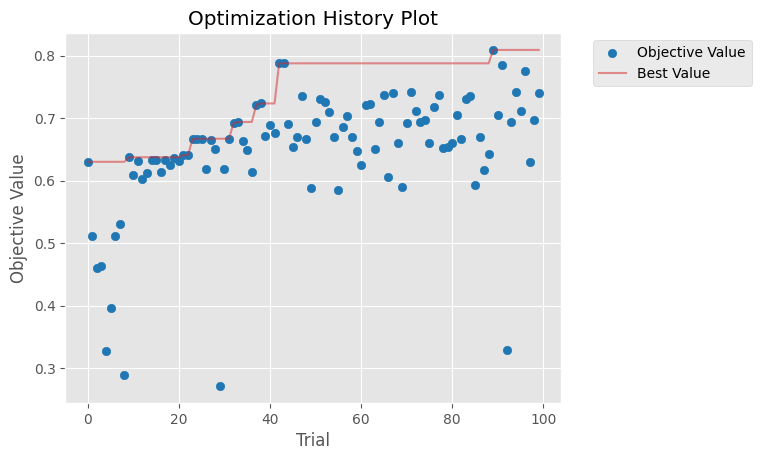
\includegraphics[width=0.8\textwidth]{../img/OptimizationHistory.png}
  \caption{Historia de optimizacion del F1-Score}\label{fig:decison-tree-optimization-history}
\end{figure}

En la Figura 1 se explica la evolucion de la metrica objetivo que fue el F1-Score a lo largo de las 100 corridas.
Se puede apreciar la tendencia a la alza de la mejor puntuacion pero tambien se observa las variaciones en el la
metrica de forma muy dispersa a lo largo de las pruebas.
La mejor puntuacion fue encontrada en la corrida 89, la cual fue la que genero el mejor F1-Score de 0.8092, las otras dos
mejores fueron encontradas alrededor de las pruebas entre 40 y 50.

\begin{figure}[H]
  \centering
  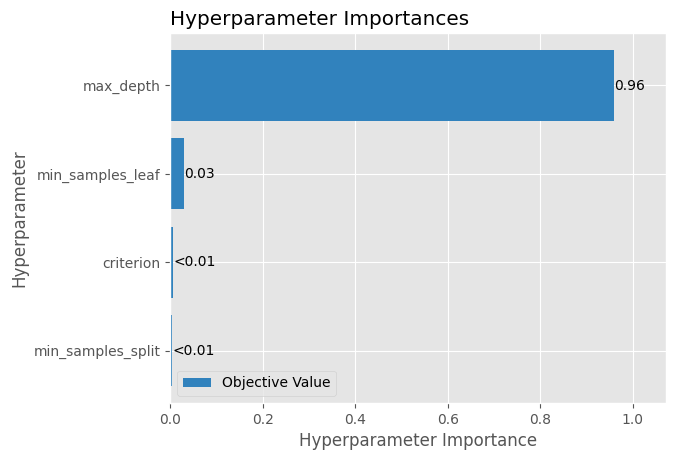
\includegraphics[width=0.8\textwidth]{../img/HyperparameterImportance.png}
  \caption{Importancia de los hiperparametros}\label{fig:decison-tree-hyperparameter-importance}
\end{figure}

En la Figura 2 se retrata cuales fueron los hiperparametros que tuvieron mas incidencia para contribuir
con la mejora de la metrica objetivo. En este caso como podemos observar la profundidad maxima tiene una
importancia mucho mas grande que las demas.
En este orden se dice que el parametro mas importante es el max_depth,
seguido por el min_samples_leaf, el min_samples_split y el criterion.

\begin{figure}[H]
  \centering
  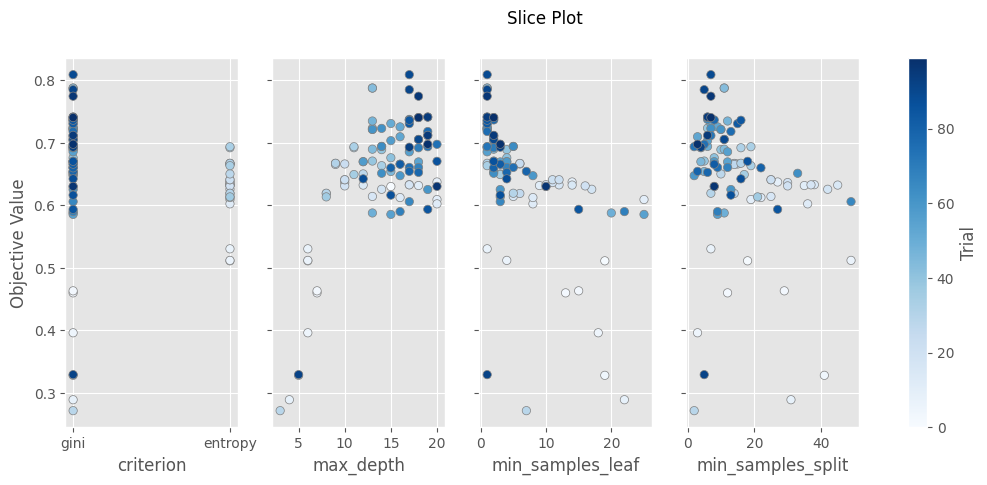
\includegraphics[width=0.8\textwidth]{../img/SliceDecisionTree.png}
  \caption{Relaciones entre hiperparametros y la metrica objetivo}\label{fig:decison-tree-slice}
\end{figure}

En la Figura 3 se muestran como los hiperparametros optimizados interactuan entre si para generar el mejor F1-Score.
En esta grafica podemos ver la tendencia de cada uno de los parametros
a cambiar su valor dentro del rango utilizado lo largo de las pruebas.
Se puede observar como alguna de estas tienden a quedarse en cierto grupo de valores,
en el caso de Gini, se ve como se utiliza mas que el valor de Entropy, asi como min_samples_leaf y min_samples_split
tienden a quedarse en valores del lado medio-bajo y finalmente el max_depth tiende a utilizar valores altos.

\begin{figure}[H]
  \centering
  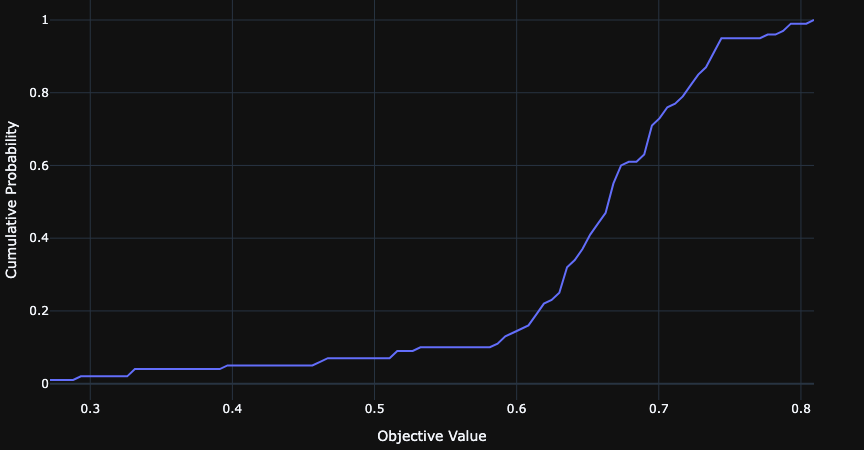
\includegraphics[width=0.8\textwidth]{../img/EDFDecisionTree.png}
  \caption{Distribucion del valor objetivo}\label{fig:edf-decision-tree}
\end{figure}

La Figura 4 es una grafica de distribucion del valor objetivo que fue el F1-Score, se observa que
la puntuacion estuvo en un rango entre alrededor de 0.3 y 0.8, siendo el 0.8 el mejor valor encontrado.
Ademas de eso se aprecia como la mayoria de pruebas tuvieron una puntuacion entre 0.6 y 0.8,
dando como resultado que con Optuna se encontraron buenos resultados en la mayoria de pruebas.

\begin{figure}[H]
  \centering
  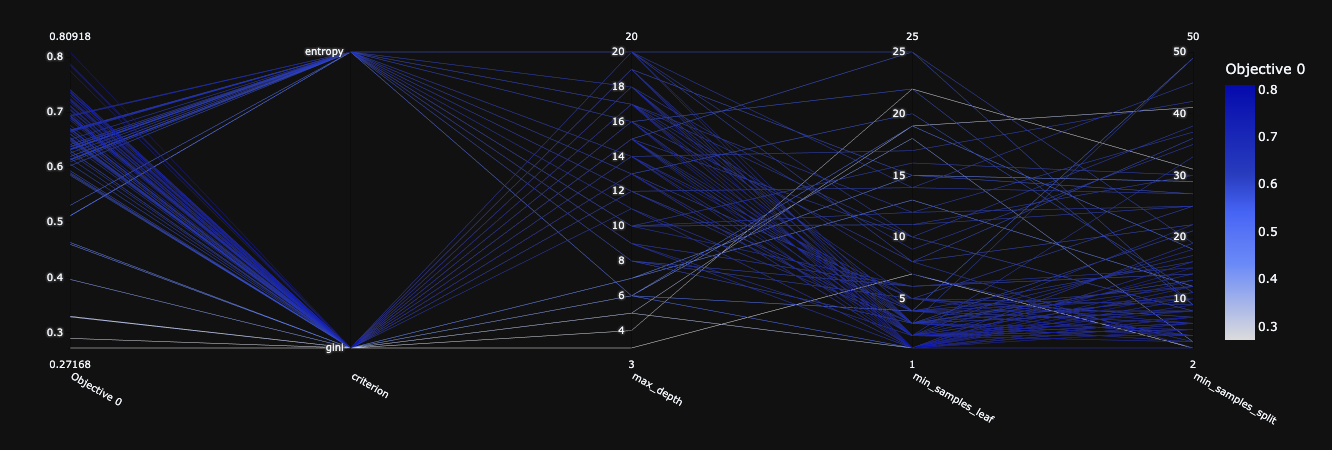
\includegraphics[width=1\textwidth]{../img/ParallelDecisionTree.png}
  \caption{Coordenadas paralelas: relación entre hiperparámetros y F1-macro}\label{fig:parallel-decision-tree}
\end{figure}

En la Figura 5 se observa que las mejores corridas por F1-macro (0.79 - 0.81)
se concentran en combinaciones con max_depth alto (13 - 17), min_samples_leaf de 1, min_samples_split (7 - 12)
y criterion de gini. Esto sugiere que el modelo se beneficia de árboles relativamente profundos con hojas pequeñas,
regulados por un umbral de división moderado. Al aumentar min_samples_leaf por encima de 1 o al reducir mucho la profundidad,
el desempeño tiende a degradarse. Asimismo, gini domina sobre entropy en este problema,
consistente con los tres mejores resultados encontrados del Cuadro 5.

\subsubsection{Comparacion de las mejores arquitecturas con particiones diferentes}

En esta seccion se comparan las tres mejores arquitecturas que se muestran en el Cuadro 5 y se evaluan
mediante 10 corridas independientes, generando particiones diferentes para cada corrida manteniendo la
proporcion definida en la funcion `split_dataset' y calculando diferentes metricas
como el F1-Score, accuracy y tasa de falsos positivos para todas las evaluaciones.
Finalmente se recopilaron todos los resultados, y se calculo las medias
y desviaciones estandar de cada una de las arquitecturas y sus corridas.

Para poder lograr el objetivo de esta seccion se guardaron los resultados de las tres mejores arquitecturas
en una lista para su uso posterior, este contenia los parametros, posicion y F1-Score de cada una de las arquitecturas.
Despues se definio la funcion `evaluate_dt_architecture_multiple_runs' la cual va estar encargada de:

\begin{itemize}
  \item Recibir los parametros de la arquitectura a evaluar necesarias para la funcion `DecisionTreeClassifier' de Scikit Learn
    asi como el numero de corridas a realizar por arquitectura y semillas si es necesario para reproducibilidad.
  \item Se itera sobre el numero de corridas y se generan las nuevas particiones por medio de la funcion `split_dataset'
  \item Se entrena el arbol de decision con los parametros recibidos y las nuevas particiones
  \item Se generan las predicciones por medio de la particion de prueba
  \item Se evalua y se obtiene el F1-Score Macro, F1-Score por clase, accuracy y
    tasa de falsos positivos para todas las evaluaciones, siendo estos
    guardados en una lista individualmente
  \item Se retorna un diccionario con los resultados de las metricas calculadas como
    numero de corridas, parametros, todos los F1-Score, accuracy, tasa de falsos positivos y matriz de confusion,
    ademas de las estadisticas como promedio y desviaciones de las metricas generadas.
\end{itemize}

Las metricas fueron calculadas mediante las funciones de Scikit Learn `f1_score', `accuracy_score', `precision_recall_fscore_support' y `confusion_matrix'.

Para el calculo de la tasa de falsos positivos se utilizo la formula:

\[
  FPR = \frac{FP}{FP + TN}
\]

Donde FP es el numero de falsos positivos y TN es el numero de verdaderos negativos.
Se utilizo la funcion `confusion_matrix' de Scikit Learn para obtener
la matriz de confusion y calcular los valores de FP y TN.

En los siguientes Cuadros 7, 8 y 9, se muestran las corridas realizadas y sus metricas.

\begin{table}[H]
  \centering
  \begin{tabular}{c c c c}
    \hline
    Corrida & F1 & Accuracy & FPR \\
    \hline
    1  & 0.7639 & 0.9988 & 0.0001 \\
    2  & 0.7294 & 0.9982 & 0.0001 \\
    3  & 0.7188 & 0.9982 & 0.0001 \\
    4  & 0.6905 & 0.9980 & 0.0002 \\
    5  & 0.7014 & 0.9981 & 0.0002 \\
    6  & 0.7413 & 0.9983 & 0.0001 \\
    7  & 0.7452 & 0.9982 & 0.0001 \\
    8  & 0.7432 & 0.9985 & 0.0001 \\
    9  & 0.8402 & 0.9984 & 0.0001 \\
    10 & 0.6797 & 0.9981 & 0.0002 \\
    \hline
  \end{tabular}
  \caption{Resultados – Arquitectura 1}
  \label{tab:corridas_arq1}
\end{table}

El Cuadro 7 exhibe como la Arquitectura 1 que era la que obtuvo la mejor puntuacion, sigue mejorando un poco
mas con estas particiones realizadas, inclusive llegando a obtener un F1-Score de 0.8402, siendo este un mejor resultado
al inicial con Optuna que se obtuvo de 0.8092.

\begin{table}[H]
  \centering
  \begin{tabular}{c c c c}
    \hline
    Corrida & F1 & Accuracy & FPR \\
    \hline
    1  & 0.7200 & 0.9979 & 0.0002 \\
    2  & 0.7110 & 0.9978 & 0.0002 \\
    3  & 0.6552 & 0.9972 & 0.0003 \\
    4  & 0.6768 & 0.9978 & 0.0002 \\
    5  & 0.6416 & 0.9981 & 0.0002 \\
    6  & 0.6390 & 0.9976 & 0.0002 \\
    7  & 0.6400 & 0.9978 & 0.0002 \\
    8  & 0.6782 & 0.9977 & 0.0002 \\
    9  & 0.6988 & 0.9976 & 0.0002 \\
    10 & 0.7262 & 0.9978 & 0.0002 \\
    \hline
  \end{tabular}
  \caption{Resultados – Arquitectura 2}
  \label{tab:corridas_arq2}
\end{table}

\begin{table}[H]
  \centering
  \begin{tabular}{c c c c}
    \hline
    Corrida & F1 & Accuracy & FPR \\
    \hline
    1  & 0.6737 & 0.9976 & 0.0002 \\
    2  & 0.6167 & 0.9974 & 0.0003 \\
    3  & 0.6483 & 0.9975 & 0.0002 \\
    4  & 0.7159 & 0.9974 & 0.0002 \\
    5  & 0.7049 & 0.9977 & 0.0002 \\
    6  & 0.6719 & 0.9973 & 0.0002 \\
    7  & 0.7013 & 0.9977 & 0.0002 \\
    8  & 0.6717 & 0.9972 & 0.0003 \\
    9  & 0.6704 & 0.9977 & 0.0002 \\
    10 & 0.6486 & 0.9970 & 0.0003 \\
    \hline
  \end{tabular}
  \caption{Resultados – Arquitectura 3}
  \label{tab:corridas_arq3}
\end{table}

En cuanto al Cuadro 8 y 9 al ser arquitecturas encontradas con configuracion identica se tienen resultados similares,
en este caso a diferencia de la primera arquitectura no se mejoro su F1-Score inicial de 0.7877.

En general todas las particiones obtuvieron metricas buenas inclusive en casi todos los falsos postivos tienen valores
muy bajos y los F1-Score por clase tambien estan cerca de 1, dando a entender que es posible que obtengan
pocas falsas detecciones y puedan clasificar en su mayoria correctamente las clases.

Para generar un resumen de todos los resultados y calcular las medias y desviaciones estandar de las metricas se genero una logica
en el notebook la cual esta encargada de utilizar todos los resultados guardados previamente de la funcion `evaluate_dt_architecture_multiple_runs'
que contiene una lista de los resultados de todas las evaluaciones, conteniendo los momentos estadisticos de
cada una de las metricas utilizadas para cada corrida por arquitectura, asi como los parametros utilizados para cada corrida.
Siguientemente la logica genera una tabla y unos graficos para visualizaion de la distribucion y valores de las medias, ademas de la desviacion estandaar
para cada arquitectura y sus corridas para una mejor comparacion.

\begin{table}[ht]
  \centering
  \tiny
  \begin{tabular}{lcccc}
    \hline
    Arquitectura & F1-macro Media & F1-macro Desviación Estandar & FPR Media & FPR Desviación Estandar \\
    \hline
    \#1 & 0.7353 & 0.0431 & 0.0001 & 0.0000 \\
    \#2 & 0.6787 & 0.0323 & 0.0002 & 0.0000 \\
    \#3 & 0.6723 & 0.0284 & 0.0002 & 0.0000 \\
    \hline
  \end{tabular}
  \caption{Resultados de las Corridas con Particiones Diferentes}
  \label{tab:corridas_part_dt}
\end{table}

\begin{figure}[H]
  \centering
  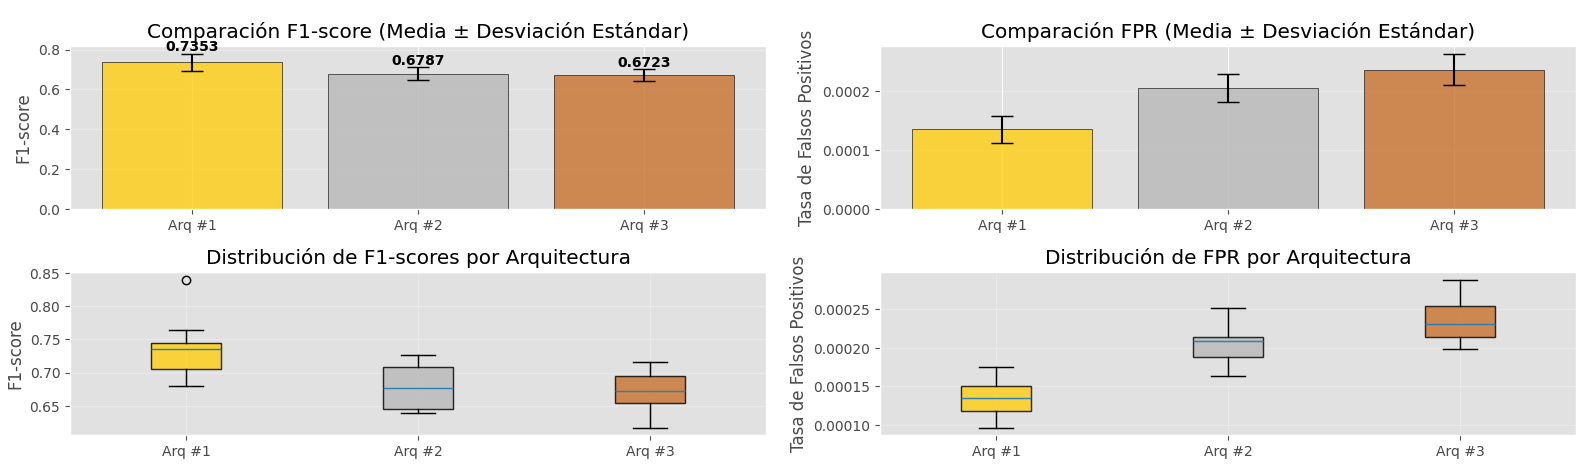
\includegraphics[width=1\textwidth]{../img/ComparacionPartArqui.png}
  \caption{Comparacion de las Arquitectura con Particiones Diferentes}\label{fig:partition-architectures-decision-tree}
\end{figure}

En el Cuadro 10 y la Figura 6 se muestran los resultados generales por arquitectura para todas las 10 corridas realizadas para cada una.
En esta se reporta la media y desviacion para las metricas que se utilizaron de F1-Score macro y tasa de falsos positivos.

En base al Cuadro 10 y la Figura 6 se pueden generar varias conclusiones de acuerdo a las arquitecturas encontradas:

\begin{itemize}
  \item La Arquitectura 1 es la que obtiene el mejor F1-Score macro y tasa de falsos positivos. Por ende
    sigue demostrando que es la mejor arquitectura en comparacion a las otras dos arquitecturas.
  \item La Arquitectura 2 y 3 al tener los mismos parametros son similares pero tienen una menor desviacion en sus resultados
    dando a entender que son un poco mas estables en sus resultados, la arquitectura 1 parece ser mas dispersa.
  \item Todas las arquitecturas presentan una tasa de falsos positivos muy baja, siendo este un buen resultado
    para el problema de deteccion de intrusos, ya que un aspecto importante es que se tengan pocas falsas detecciones
    y un sistema de este tipo sea mas robusto.
\end{itemize}

\end{document}